\chapter{Synchronization of digital records}
\label{app:DigitizerSynchronization}
Digital signal processing is often foundational to signal analysis.
Of course, application of such techniques
requires converting an analog signal to a digital record.
Efficient conversion requires
both quantization of the signal magnitude and
temporal sampling~\cite{bennett_bstj48}.
When examining the phasing between multiple digital records,
the synchronization of this temporal sampling
is of paramount importance.

This appendix discusses post-processing synchronization of digital records.
Below, Section~\ref{app:DigitizerSynchronization:temporal_sampling}
defines temporal sampling and
mentions caveats regarding nominal and actual sampling parameters.
Section~\ref{app:DigitizerSynchronization:digitization_schemes}
then discusses various digitization schemes,
highlighting which schemes allow synchronization.
Finally, Section~\ref{app:DigitizerSynchronization:phase_locked_synchronization}
details the synchronization of phase-locked digital records.


\section{Temporal sampling}
\label{app:DigitizerSynchronization:temporal_sampling}
Typically, temporal sampling of signal $x_j(t)$ occurs
at a fixed sampling rate $F_j$ such that
successive points in the digital record
are separated in time by $1 / F_j$.
Digitization begins at the trigger time $t_j[0]$ such that
the $m\ts{th}$ digitized point is sampled at time
\begin{equation}
  t_j[m] = t_j[0] + \frac{m}{F_j}.
  \label{eq:DigitizerSynchronization:timebase_generic}
\end{equation}
Ideally, the \emph{realized} sampling rate $F_j$ and trigger time $t_j[0]$
are equal to their \emph{nominal} values
$F_j^{\nom}$ and $t_j^{\nom}[0]$, respectively.
However, short-term jitter, long-term drifts, and constant offsets
often plague real-world digitization such that
$F_j \neq F_j^{\nom}$, $t_j[0] \neq t_j^{\nom}[0]$, and
\begin{equation}
  t_j[m] \neq t_j^{\nom}[0] + \frac{m}{F_j^{\nom}};
\end{equation}
that is, the actual sample times of the digital record
differ from their nominal values.
In a properly operating digitizer,
these discrepancies are typically small, and
an autospectral-density estimate (for example)
of $x_j(t)$ from its digital record
will be negligibly compromised.
When estimating the \emph{phasing}
between $x_j(t)$ and $x_{k}(t)$ for $j \neq k$, however,
identifying and correcting such timebase discrepancies
becomes paramount in importance.


\section{Which digital records can be synchronized?}
\label{app:DigitizerSynchronization:digitization_schemes}
The digitization scheme determines
whether or not digital records
$\{x_j[m]\}$ and $\{x_k[m]\}$
can be synchronized.
The cleanest, simplest, and most problem-free scheme
is to digitize $x_j(t)$ and $x_k(t)$ on the \emph{same} system
such that the actual sample rates and trigger times
of both digital records are identical
(i.e.\ $F_j = F_k$ and $t_j[0] = t_k[0]$, respectively).
However, such a scheme is not always feasible.
Further, note that multiple digitizer boards
operating in a master-slave configuration
can still suffer from trigger-time offsets,
despite nominally being part of the same digitization system.
The next-best scheme is to use phase-locked digitizers
such that
\begin{equation}
  \frac{F_j}{F_k}
  =
  \frac{F_j^{\nom}}{F_k^{\nom}}
  =
  \text{constant (for \emph{phase-locked} digitizers)},
  \label{eq:DigitizerSynchronization:phase_locked_constraint}
\end{equation}
regardless of any short-term jitter or long-term drift
in the digitizer clocks.
As shown in
Section~\ref{app:DigitizerSynchronization:phase_locked_synchronization},
the actual sampling times of phase-locked digital records
differ (at most) by a constant ``trigger offset'',
which can be compensated easily.
Finally, the least-desirable scheme
is to use free-running digitizers
such that $F_j / F_k \neq F_j^{\nom} / F_k^{\nom}$;
it may be impossible to synchronize records
from free-running digitizers.
While the below discussion considers
synchronization via post-processing,
it should be noted for completeness
that hardware solutions for synchronization also exist
\cite{stillerman_fed10}.


\section{Synchronization of phase-locked digital records}
\label{app:DigitizerSynchronization:phase_locked_synchronization}
This section details the synchronization of phase-locked digital records.
Specifically, Section~\ref{app:DigitizerSynchronization:phase_locked_synchronization:trigger_offset}
defines the ``trigger offset'' between phase-locked digital records, and
Section~\ref{app:DigitizerSynchronization:phase_locked_synchronization:trigger_offset_effect}
discusses the phase bias produced by a finite trigger offset.
Section~\ref{app:DigitizerSynchronization:phase_locked_synchronization:trigger_offset_estimates}
describes methods for estimating the trigger offset.
Then, using standard techniques~\cite[Sec.~4.5]{oppenheim},
the trigger offset can be compensated easily in post-processing,
even if the offset is a non-integer multiple of the sample spacing.


\subsection{The ``trigger offset''}
\label{app:DigitizerSynchronization:phase_locked_synchronization:trigger_offset}
Phase-locked digitizers may suffer from a deleterious ``trigger offset''.
To see this, consider two digitizers $j$ and $k$.
Assume that the digitizers have different nominal trigger times
$t_j^{\nom}[0] \neq t_k^{\nom}[0]$ but
the same nominal sampling rate
$F_j^{\nom} = F_k^{\nom}$.
(If the digitizers have different nominal sampling rates, however,
the records from one of the digitizers
can be digitally resampled~\cite[Sec.~4.6]{oppenheim}
with the sampling rate of the other digitizer, and
then the presentation below proceeds unchanged).
Because the nominal trigger times of digitizers $j$ and $k$ differ,
their $m\ts{th}$ nominal timestamps also differ,
i.e.\ $t_j^{\nom}[m] \neq t_k^{\nom}[m]$.
Instead, $t_j^{\nom}[m] = t_k^{\nom}[n]$, where
\begin{equation}
  n
  =
  m
  +
  F_j^{\nom}
  \left(
    t_j^{\nom}[0]
    -
    t_k^{\nom}[0]
  \right),
  \label{eq:DigitizerSynchronization:nominal_timebase_index_relation}
\end{equation}
and the equality of the nominal sampling rates has been utilized.
Now, for digitizer $j$ define
$\delta t_j = t_j[0] - t_j^{\nom}[0]$
to be the difference between the actual and nominal trigger times,
$\delta F_j = F_j - F_j^{\nom}$
to be the difference between the actual and nominal sampling rates, and
$\bar{\delta F_j} = \delta F_j / F_j^{\nom}$
to be the normalized difference between the actual and nominal sampling rates
($|\bar{\delta F_j}| \ll 1$).
Similar definitions apply for digitizer $k$.
Because the digitizers satisfy the phase-locked constraint
(\ref{eq:DigitizerSynchronization:phase_locked_constraint}),
\begin{equation}
  \bar{\delta F_j} = \bar{\delta F_k}.
  \label{eq:DigitizerSynchronization:phase_locked_normalized_sample_rate_deviations}
\end{equation}
(Note that equality
(\ref{eq:DigitizerSynchronization:phase_locked_normalized_sample_rate_deviations})
holds even if the nominal sampling rates are different).
Then, to first order in $\bar{\delta F_j}$,
the actual sampling times $t_j[m]$
are related to the nominal sampling times $t_j^{\nom}[m]$ via
\begin{equation}
  t_j[m]
  \approx
  t_j^{\nom}[m]
  +
  \delta t_j
  -
  \frac{m \cdot \bar{\delta F_j}}{F_j^{\nom}}.
  \label{eq:DigitizerSynchronization:timebase_actual_vs_nominal}
\end{equation}
Thus, trigger-time discrepancy $\delta t_j$
produces a constant offset
between the actual and nominal sampling times of digitizer $j$, while
sampling-rate discrepancy $\delta F_j$
produces a linear ramp
between the actual and nominal sampling times of digitizer $j$.

Now, in some situations it is of the utmost importance
that the actual sampling times of digitizers $j$ and $k$ align.
(Inferring the spatial structure of a signal from its phasing
between two spatially separated sensors is one such example).
The \emph{nominal} sampling times are aligned via
(\ref{eq:DigitizerSynchronization:nominal_timebase_index_relation}), but
any remaining discrepancy between the \emph{actual} sampling times is
\begin{align}
  \delta t_{\trig}
  &=
  t_j[m] - t_k[n]
  \notag \\
  &=
  \left( \delta t_j - \delta t_k \right)
  +
  \bar{\delta F_j} \left( t_j^{\nom}[0] - t_k^{\nom}[0] \right);
  \label{eq:DigitizerSynchronization:trigger_offset}
\end{align}
this situation is shown schematically in
Figure~\ref{fig:DigitizerSynchronization:trigger_offset_schematic}.
Here, the first term on the right-hand side of
(\ref{eq:DigitizerSynchronization:trigger_offset})
corresponds to the difference between
trigger-time discrepancies of each digitizer, while
the second term on the right-hand side
corresponds to the relative sampling-rate discrepancy
weighted by the difference in nominal trigger times.
As both effects are related to triggering,
this timestamp discrepancy is referred to as
the ``trigger offset'' $\delta t_{\trig}$.
Note that $\delta t_{\trig}$ is a single, constant value
for any given pair of phase-locked digital records.

\begin{figure}
  \centering
  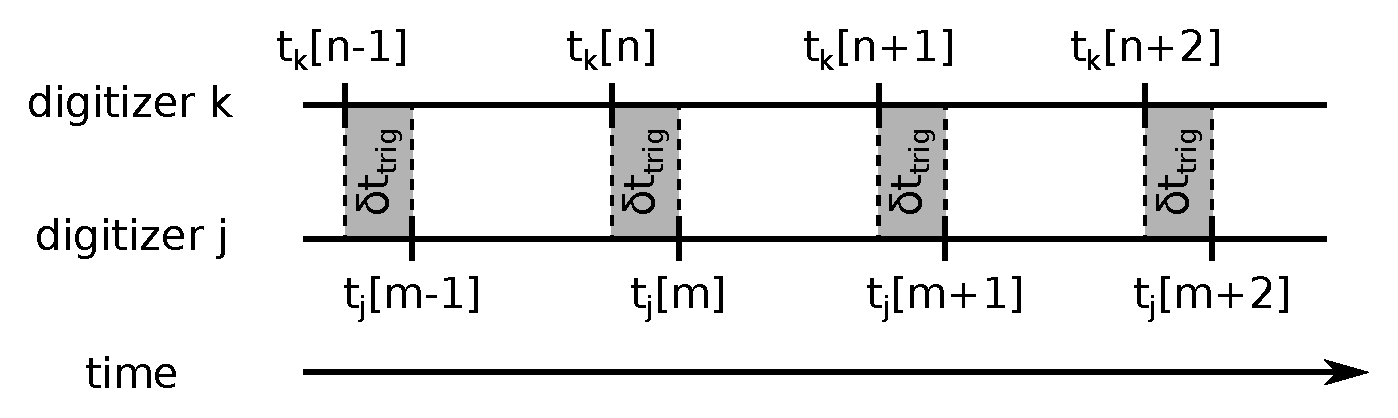
\includegraphics[width = \textwidth]{%
    Appendices/DigitizerSynchronization/figs/trigger_offset_schematic.pdf}
  \caption[``Trigger offset'' between phase-locked digitizers]{%
    The ``trigger offset'' $\delta t_{\trig}$ between phase-locked digitizers.
    Here, the $n\ts{th}$ nominal sampling time of digitizer $k$ equals
    the $m\ts{th}$ nominal sampling time of digitizer $k$
    (i.e.\ $t_j^{\nom}[m] = t_k^{\nom}[n]$), where
    $n$ and $m$ are related via
    (\ref{eq:DigitizerSynchronization:nominal_timebase_index_relation}).
    However, a finite trigger offset
    (\ref{eq:DigitizerSynchronization:trigger_offset})
    produces a discrepancy between the \emph{actual} sampling times
    of the two digitizers (i.e.\ $t_j[m] \neq t_k[n]$),
    which can bias phase measurements, as discussed in
    Section~\ref{app:DigitizerSynchronization:phase_locked_synchronization:trigger_offset_effect}.
  }
\label{fig:DigitizerSynchronization:trigger_offset_schematic}
\end{figure}


\subsection{Effect of the trigger offset}
\label{app:DigitizerSynchronization:phase_locked_synchronization:trigger_offset_effect}
The trigger offset (\ref{eq:DigitizerSynchronization:trigger_offset})
biases the measured phasing between the digital records.
To see this, let $x_j(t)$ be a coherent mode
of angular frequency $\omega$ such that
the corresponding digital record is
\begin{align}
  x_j[m]
  &=
  x_j(t_j[m])
  \notag \\
  &\propto
  X_j(\omega) e^{i \omega t_j[m]}
  \notag \\
  &=
  |X_j(\omega)| e^{i \{ \alpha_j(\omega) + \omega t_j[m]\}},
\end{align}
where $|X_j(\omega)|$ is the Fourier amplitude and
$\alpha_j(\omega)$ is the Fourier phase.
(Here, the Fourier-transform kernel is $\propto e^{-i \omega t}$ and
the inverse Fourier-transform kernel is $\propto e^{i \omega t}$,
in accord with the NumPy implementation
of the fast Fourier transform (FFT)~\cite{numpy_fft};
if the opposite convention is used for FFT computations,
then the substitution $\delta t_{\trig} \rightarrow -\delta t_{\trig}$
should be made in equations
(\ref{eq:DigitizerSynchronization:measured_phase_difference}),
(\ref{eq:DigitizerSynchronization:trigger_offset_estimate_apriori_phase}), and
(\ref{eq:DigitizerSynchronization:trigger_offset_estimate_frequency_swept})).
Then, after aligning \emph{nominal} sampling times via
(\ref{eq:DigitizerSynchronization:nominal_timebase_index_relation}),
the \emph{measured} phase difference $\Delta \alpha_{\meas}$
between digital records $\{x_j[m]\}$ and $\{x_k[n]\}$ is
\begin{align}
  \Delta \alpha_{\meas}
  &=
  \arg\left(
    x_k^*[n]
    \cdot
    x_j[m]
  \right)
  \notag \\
  &=
  \left[
    \alpha_j(\omega)
    -
    \alpha_k(\omega)
  \right]
  +
  \omega
  \left(
    t_j[m] - t_k[n]
  \right)
  \notag \\
  &=
  \Delta \alpha(\omega)
  +
  \left( \omega \cdot \delta t_{\trig} \right),
  \label{eq:DigitizerSynchronization:measured_phase_difference}
\end{align}
where $\Delta \alpha(\omega) = \alpha_j(\omega) - \alpha_k(\omega)$
is the true phase difference and
$\delta t_{\trig}$ is defined in
(\ref{eq:DigitizerSynchronization:trigger_offset}).
Thus, non-zero trigger offset $\delta t_{\trig}$ biases
the measured phase difference $\Delta \alpha_{\meas}$
away from the true phase difference $\Delta \alpha$.
The above argument readily extends to broadband signals.


\subsection{Estimating the trigger offset}
\label{app:DigitizerSynchronization:phase_locked_synchronization:trigger_offset_estimates}
Clearly, a finite trigger offset is undesirable.
In some situations, it is possible
to estimate the trigger offset.
Then, using standard techniques~\cite[Sec.~4.5]{oppenheim},
the trigger offset can be compensated easily in post-processing,
even if the offset is a non-integer multiple of the sample spacing.

If the true phase difference $\Delta \alpha(\omega)$
is known \emph{a priori} (from e.g.\ another measurement),
solving for $\delta t_{\trig}$ in
(\ref{eq:DigitizerSynchronization:measured_phase_difference})
yields an estimated trigger offset
\begin{equation}
  \delta t_{\trig}
  =
  \frac{\Delta \alpha_{\meas}(\omega) - \Delta \alpha(\omega)}{\omega}.
  \label{eq:DigitizerSynchronization:trigger_offset_estimate_apriori_phase}
\end{equation}
Although \emph{a priori} knowledge of $\Delta \alpha$ may make
(\ref{eq:DigitizerSynchronization:trigger_offset_estimate_apriori_phase})
seem rather academic,
it does find real-world application.
For example, imagine the signals from
a regularly spaced array of channels
are digitized across multiple digitizer boards.
The intra-board trigger offsets are negligible
such that the true phase difference $\Delta \alpha$
can be accurately estimated from
adjacent channels digitized on the same board;
comparing this estimate of $\Delta \alpha$
to the measured phase difference $\Delta \alpha_{\meas}$
between adjacent channels digitized on different boards
via (\ref{eq:DigitizerSynchronization:trigger_offset_estimate_apriori_phase})
then yields an estimate of the trigger offset between the boards.
This methodology is used to estimate the trigger offset
between the two boards of the \diiid\space PCI digitizer.

In addition to requiring \emph{a priori} knowledge
of the true phase difference $\Delta \alpha$,
trigger-offset estimate
(\ref{eq:DigitizerSynchronization:trigger_offset_estimate_apriori_phase})
also suffers from aliasing.
That is, $\Delta \alpha_{\meas}$ is only measured modulo $2 \pi$ such that
(\ref{eq:DigitizerSynchronization:trigger_offset_estimate_apriori_phase})
specifies an infinite set of potential trigger offsets,
with adjacent values spaced by $2 \pi / \omega$.
This is particularly troublesome for ``large'' trigger offsets.

Under certain circumstances, the trigger offset
can be estimated in an alternative, alias-free manner.
For example, consider a coherent mode
with time-dependent angular frequency $\omega(t)$.
If the angular frequency ramps linearly in time
(i.e.\ $\dot{\omega} = d\omega / dt = \text{constant}$) and
the true phase difference $\Delta \alpha$
does \emph{not} vary in time,
taking the time derivative of
(\ref{eq:DigitizerSynchronization:measured_phase_difference}) and
solving for $\delta t_{\trig}$ yields
\begin{align}
  \delta t_{\trig}
  =
  \frac{1}{\dot{\omega}}
  \frac{d\left[ \Delta \alpha_{\meas}(\omega) \right]}{dt}
  =
  \frac{d\left[ \Delta \alpha_{\meas}(\omega) \right]}{d\omega}.
  \label{eq:DigitizerSynchronization:trigger_offset_estimate_frequency_swept}
\end{align}
Because
(\ref{eq:DigitizerSynchronization:trigger_offset_estimate_frequency_swept})
depends on the derivative of $\Delta \alpha_{\meas}$,
it is an alias-free estimate of the trigger offset.
Further,
(\ref{eq:DigitizerSynchronization:trigger_offset_estimate_frequency_swept})
does \emph{not} require \emph{a priori} knowledge
of the true phase difference $\Delta \alpha$
(other than requiring that it be constant in time).
This methodology is used to estimate the trigger offset
between \diiid's two toroidally separated interferometers.


\bibliographystyle{plainurl}
\bibliography{references}
